\begin{frame}
  \frametitle{Por que EDEs?}
    \begin{empheq}[box={\Garybox[En ocaciones]}]{align*}
        EDO+ruido=Mejor \text{ } modelo
    \end{empheq}
    \begin{overlayarea}{\textwidth}{.8\textheight}
        \begin{columns}
            \column{.55\textwidth}
            \only<2-3>{
                \begin{exampleblock}{Crecimiento de Poblaciones}
                    $$
                        \frac{dN}{dt}=a(t)N(t) \qquad N_0=N(0)=cte.
                    $$
                \end{exampleblock}
            }
            \only<4-6>{
            \begin{exampleblock}{Circuitos Eléctricos}
                \begin{align*}
                   &L\cdot Q''(t)+
                    R\cdot Q'(t)+
                    \frac{1}{C}\cdot Q(t)
                        =F(t)
                    \\
                   &Q(0)=Q_0\\
                   &Q'(0)=I_0
                \end{align*}
            \end{exampleblock}
        }
        \column{.58\textwidth}
        \only<3>{
            \begin{empheq}[box=\shadowbox*]{equation*}
                a(t)=r(t)+"ruido"
            \end{empheq}
        }
        \only<5-6>{
            %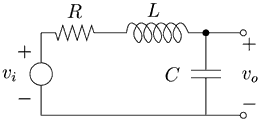
\includegraphics[width=\textwidth]{./images/CircuitRLC.png}
            \begin{circuitikz}[american voltages]
                \draw (0,0)
                to[sV,v=$F(t)$] (0,2) % The voltage source
                to[R=$R$, i^>=$i(t)$] (2,2) % The resistor
                to[L=$L$] (4,2)
                to[C=$C$] (4,0)--(0,0) ;
            \end{circuitikz}
        }
        \only<6>{
            \begin{empheq}[box=\shadowbox*]{equation*}
                F(t)=G(t)+"ruido"
            \end{empheq}
        }
        \end{columns}
    \end{overlayarea}
\end{frame}
%%%%%%%%%%%%%%%%%%%%%%%%%%%%%%%%%%%%%%%%%%%%%%%%%%%%%%%%%%%%%%%%%%%%%%%%%%%%%%%%%%
\begin{frame}
    \frametitle{Para fijar ideas}
    \begin{empheq}[box={\Garybox[Ejemplo]}]{align*}
        dN(t) = aN(t)dt
    \end{empheq}
    \begin{overlayarea}{\textwidth}{.3\textheight}
        \begin{columns}
            \column{.5\textwidth}
                \only<2->{
                    \begin{block}{Perturba sobre $[t, t+dt)$}
                        \only<3->{
                            $$
                              a dt
                              \rightsquigarrow
                              a dt + \sigma dB(t)
                            $$
                        }
                    \end{block}
               }
            \column{.5\textwidth}
        \only<4->{
            \begin{exampleblock}{obten una EDE}
              $$
               dN(t) = aN(t)dt + \sigma N(t) dB(t)
              $$
            \end{exampleblock}
        }
        \end{columns}
    \end{overlayarea}
    \begin{overlayarea}{\textwidth}{.7\textheight}
        \centering
            \resizebox{0.45\textwidth}{!}{%
            \only<5>{
                \begin{tikzpicture}
                    \begin{axis}[%
                     line width=1.0pt,
                     mark size=1.0pt
                     ]%
                         \addplot[color=blue]%
                         table [%
                           x index = {0},
                           y index = {1} %
                       ]{\mydata};
                       \addplot[domain=0:5, samples=100]{1.5*exp(x)};
                    \end{axis}
                \end{tikzpicture}
         }
        }
    \end{overlayarea}
\end{frame}